\section{Geometric Visualization}

\textbf{General Equation}

\bigskip
\begin{equationbox}{$\boldsymbol{XY-}$plane}
\textbf{Definition:} The $xy-$plane (Cartesian plane) is used to plot rectangular coordinates $(x, y)$.

\begin{center}
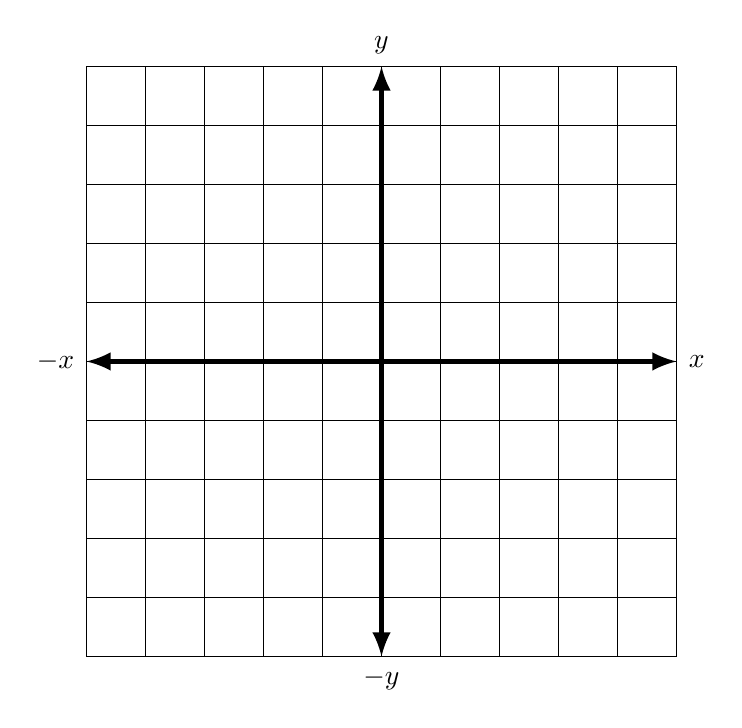
\begin{tikzpicture}[scale=0.75]
\fill[white] (0,0) rectangle (10,10);
\draw (0,0) grid (10,10);
\draw[latex-latex, line width=2pt] (5,0) node[below] {$-y$} -- (5,10) node[above] {$y$};
\draw[latex-latex, line width=2pt] (0,5) node[left] {$-x$} -- (10,5) node[right] {$x$};
\end{tikzpicture}
\end{center}
\end{equationbox}

\bigskip
\begin{enumerate}[labelindent=*,style=multiline,leftmargin=*,label=\textbf{Example \arabic*:}]
\item An northward facing arrow is rotated $45^\circ$ counterclockwise, then flipped vertically and horizontally. What direction is the arrow now facing?
\vfill\item Opposite sides of dice have a sum of 7. If John rolls a die three times and the sum of his rolls is 7, what is the sum of the opposite sides of the same three rolls?
\vfill\item A right isosceles triangle with a radius of 2 is rotated about its right angle to form a 3-dimensional solid. What is the volume of the resulting shape?
\end{enumerate}

\vfill
\newpage
\begin{multicols*}{2}
\begin{outline}[enumerate]
\medium

\1 If a circle is cut into regions by three lines, what is the maximum number of regions formed?

\bigskip
\textbf{Equation/Strategy:} \hrulefill

\bigskip
\textbf{Solve:}

\vfill
\2 3
\2 4
\2 5
\2 6
\2 7

\midline

\1 A square piece of paper of side length 10 is folded along its diagonal to make a triangle. The triangle is then folded symmetrically in half down the middle, resulting in another triangle. What is the perimeter of the final triangle?

\bigskip
\textbf{Equation/Strategy:} \hrulefill

\bigskip
\textbf{Solve:}

\vfill
\2 10
\2 15
\2 $10\sqrt{2}$
\2 $5+5\sqrt{2}$
\2 $10+10\sqrt{2}$

\columnbreak
\advanced

\1 The steering wheel of a boat has 4 spokes, colored red, blue, green, and purple in that order going clockwise. If the red spoke faces east when the boat is at rest, what color faces north when the wheel has rotated 2.5 times counterclockwise?

\bigskip
\textbf{Equation/Strategy:} \hrulefill

\bigskip
\textbf{Solve:}

\vfill
\2 Red
\2 Blue
\2 Green
\2 Purple
\2 Cannot be determined

\midline

\1 A roll of tape has a tube with a diameter of 10 cm and a uniform layer of tape that is 5mm. If the tape has a thickness of 1mm, what is the approximate length of the tape unraveled?

\bigskip
\textbf{Equation/Strategy:}

\bigskip
\textbf{Solve:}

\vfill
\2 157 cm
\2 314 cm
\2 1.57 cm
\2 3.14 cm
\2 15708 cm
\end{outline}
\end{multicols*}